\section{Third data set}

This section of the report is an analysis of real credit card default data, \citetitle{Cheng:2026} \cite{Cheng:2026},
from a Taiwan bank in 2005.

The data contains a snapshot of client information showing those who have defaulted on their repayments, along with their
credit limit and history of their bill amounts, re-payment amounts and outstanding payments, along with certain client demographics, such
as age, marriage status, education level and gender.

The aim for the analysis here was to develop a robust predictive model using \texttt{GAMLSS} that captures the complex dynamics in the
probability of default among credit card holders.  This question seeks to explore the efficacy of GAMLSS, which allows for the
flexible modeling of distributions and can accommodate the skewness and kurtosis inherent in financial datasets. 

This data set had been investigated by other researchers \cite{Yeh:2009} so we have a baseline for comparing our results against other
methodologies.

A note in here; the size and poor correlations of the explanatory variables with the response meant that the analysis and
fitting stages were very time consuming and error prone.  

\subsection{Data Schema}

\begin{verbatim}
# Variable Name Role	Type	  Demographic	      Description	Units	Missing Values
# ID           ID	  Integer				                              no
# X1	       Feature	  Integer		                LIMIT_BAL		      no
# X2	       Feature	  Factor	  Sex	            SEX		              no
# X3	       Feature	  Factor	  Education Level	EDUCATION		      no
# X4	       Feature	  Factor	  Marital Status	MARRIAGE		      no
# X5	       Feature	  Integer	  Age	            AGE		              no
# X6	       Feature	  Double		                PAY_0		          no
# X7	       Feature	  Double		                PAY_2		          no
# X8	       Feature	  Double		                PAY_3		          no
# X9	       Feature	  Double		                PAY_4		          no
# X10	      Feature	  Double		                PAY_5		          no
# X11	      Feature	  Double		                PAY_6		          no
# X12	      Feature	  Double		                BILL_AMT1		      no
# X13	      Feature	  Double		                BILL_AMT2		      no
# X14	      Feature	  Double		                BILL_AMT3		      no
# X15	      Feature	  Double		                BILL_AMT4		      no
# X16	      Feature	  Double		                BILL_AMT5		      no
# X17	      Feature	  Double		                BILL_AMT6		      no
# X18	      Feature	  Double		                PAY_AMT1		      no
# X19	      Feature	  Double		                PAY_AMT2		      no
# X20	      Feature	  Double		                PAY_AMT3		      no
# X21	      Feature	  Double		                PAY_AMT4		      no
# X22	      Feature	  Double		                PAY_AMT5		      no
# X23	      Feature	  Double		                PAY_AMT6		      no
# Y	          Target	  Binary		                default.payment.next.month		no
\end{verbatim}

\subsubsection{Preliminary Analysis}

The data are clean and reliable with no missing values.  The csv file contains 30000 rows of data with:
one identity column; 23 explanatory variables and; the response
variable \texttt{default.payment.next.month}.


\begin{figure}[H]
  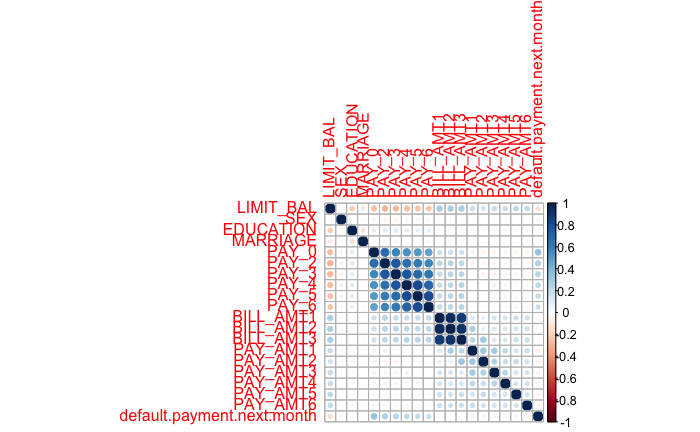
\includegraphics{q3_data_corr.png}
  \caption{Correlation analysis of the credit card default variables}
\end{figure}

The correlation between any of the variables is quite low, making the building of a robust model difficult.

\subsection{Statistical Model}

Our baseline BI model is build with all explanatory variable:
\begin{verbatim}
mbi <- gamlss(default.payment.next.month~LIMIT\_BAL+PAY\_0+PAY\_2+PAY\_3+PAY\_4+PAY\_5+PAY\_6+AGE+
                factor(EDUCATION)+factor(SEX)+factor(MARRIAGE)+BILL\_AMT1+PAY\_AMT1+BILL\_AMT2+PAY\_AMT2+
                BILL\_AMT3+PAY\_AMT3+BILL\_AMT4+PAY\_AMT4+BILL\_AMT5+PAY\_AMT5+BILL\_AMT6+PAY\_AMT6, 
              family=BI, # BI is for Binomial distribution
              data=cc\_train)
\end{verbatim}


\subsubsection{Selecting a Distribution}

The response variable \textbf{\texttt{default.payment.next.month}} is a binary value on the default event: one as 'Yes', zero as 'No'.
Binomial models are our only alternatives here. Manually fitting the different families show that the standard \textbf{Binomial Model}
\verb|BI| gives the best AIC scoring.  This is fortunate as with testing a large number of explanatory variable using stepwise
algorithms is already computationally expensive.


\subsection{Model Diagnostics}

\begin{figure}[H]
  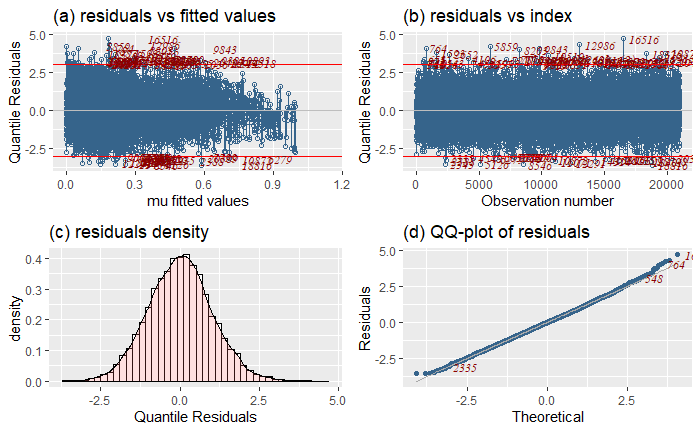
\includegraphics{q3_mbi_plot.png}
  \caption{BI residuals worm plot for credit card defaults}
\end{figure}

In this residuals analysis we start to see the problems before us.  The residuals worm plot has a high curvature and large extreme
values.

\begin{figure}[H]
  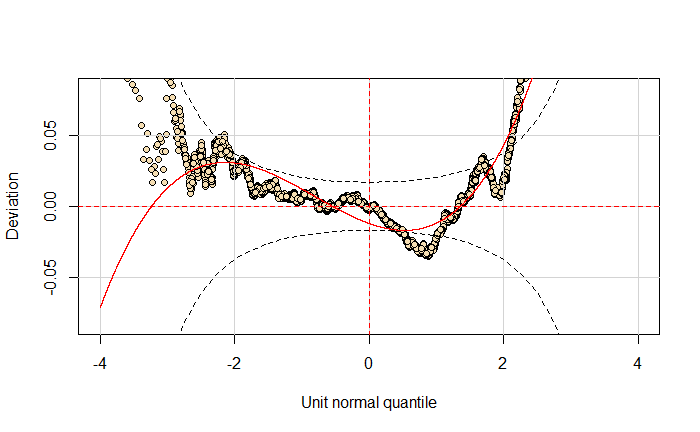
\includegraphics{q3_mbi_wp.png}
  \caption{BI residuals worm plot for credit card defaults}
\end{figure}

Using the \verb|stepGAICAll.B| function we find an improved AIC, but the worm plot is not much improved.

Using spline smoothing improves the situation markedly.

\begin{figure}[H]
  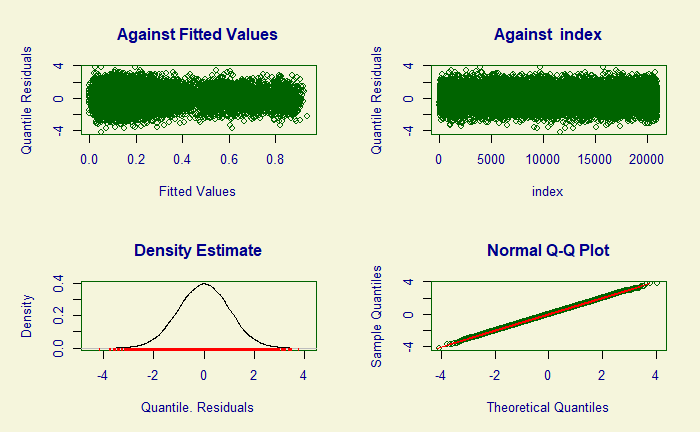
\includegraphics{q3_mbi4_plot.png}
  \caption{BI with smoothing and stepwise residuals plot}
\end{figure}

\begin{figure}[H]
  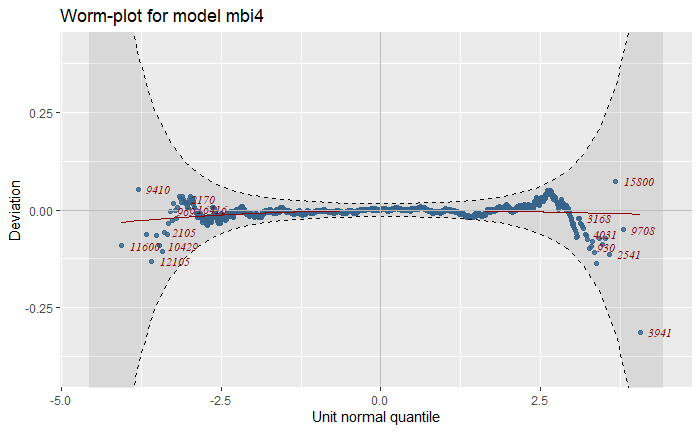
\includegraphics{q3_mbi4_wp.png}
  \caption{BI with smoothing and stepwise residuals worm plot}
\end{figure}



\subsection{Model Prediction}


\begin{verbatim}
library(pROC)
predicted_probabilities <- predict(mbi4, newdata = cc_validation, type = "response")
actual_values <- cc_validation$default.payment.next.month
roc_curve <- roc(cc_validation$default.payment.next.month, predicted_probabilities)
plot(roc_curve, main = "ROC Curve")


cor(predicted_probabilities, actual_values)
[1] 0.4489414
\end{verbatim}

\begin{figure}[H]
  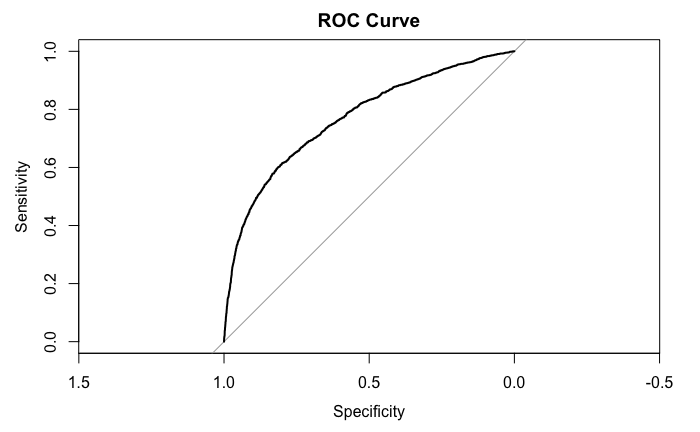
\includegraphics{q3_predict_roc.png}
  \caption{BI with smoothing and stepwise residuals worm plot}
\end{figure}

The correlation value is low.  This needs more work.
